\chapter{Sequential Circuits}
\label{chapter:Sequential Circuits}
\graphicspath{ {./chapter05/Fig} }

The preceding four chapters have focused on \textit{ combinational
circuits}, digital systems whose output depends solely on
the input.  That is,

$$output = F(input)$$

A good example of a combinational circuit is an adder.  When
the inputs 3 and 2 are applied to a 3-bit adder, the output
is always 5 regardless of what inputs were applied to the
circuit in the past. However, another whole class of
circuits remembers events in the past and adjusts
their outputs to reflect these events.

The output of a \textit{ sequential circuit} to a given input
depends on what inputs were applied in the past.  A good
example of a sequential circuit is a counter: a
digital circuit that outputs a count value, increasing
every time a ``count up" signal is asserted.  Clearly, the
same input (telling the counter to count up) may elicit
many different outputs depending on the current count
value.  A desktop PC is another good example of a
sequential circuit.  The same input (clicking a mouse) may cause an
English paper to be saved or an alien invader to be destroyed.  Thus, the
relationship between the inputs and outputs of a sequential circuit
is more complex than in a combinational circuit and needs
to be described in a fundamentally different way. In order to relate
the inputs of a sequential circuit to the output, the concept of a
state variable needs to be introduced.  In some sequential circuits, the
state of a system can be thought of as a memory of the past inputs.
In other sequential circuits
representing a process, it is best to regard the state as the current
step within that process.  The relationship between the output of
a sequential circuit is described as,

$$output = F(input, state)$$

A digital circuit which  controls a home heating furnace is examined
in order  to emphasize the differences between combinational and
sequential circuits as well as to clarify the concept of state.

When the temperature is below $T_{set}$, the furnace should be on
and when the temperature is above $T_{set}$, the furnace should be
off.  The furnace controller circuit has 1-bit of output, when
it is 0, the furnace turns off and when its output is 1, the furnace turns on.
The input to the furnace controller comes
from a temperature sensor which outputs a 0 when the temperature
is below $T_{set}$ and outputs a 1 when the temperature
is above $T_{set}$.  This behavior is captured in the graph shown
in Figure~\ref{fig:sequentialCirSimpleFurnace}.

\begin{figure}[ht]
    \center{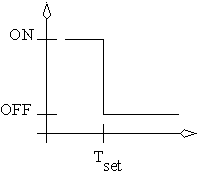
\includegraphics{SimpleFurnace}}
    \caption{A simple furnace controller for a house.}
    \label{fig:sequentialCirSimpleFurnace}
\end{figure}

The y-axis of this graph describes the state of the furnace;
the furnace is either on or off.  The x-axis describes the
temperature of the house.
If the temperature is less than $T_{set}$, then the furnace is on.
If the temperature is greater than $T_{set}$, then the furnace is off.
It should not be hard to surmise that the digital circuit required to
control the temperature is a NOT gate.  While this may seem like a
satisfactory solution to the temperature control problem, it would
perform quite poorly in practice.  It is instructive to examine why.

Assume the house was initially cold when the
furnace controller was turned on.  Clearly, the controller would turn on the furnace
and warm the house up. At some point, the temperature in the house would
warm up to $T_{set}$ causing the controller to turn off the furnace.
Because of the residual heat in the furnace the temperature may overshoot
$T_{set}$.  Soon however, the temperature would drop below $T_{set}$ causing
the controller to turn the furnace on.  This time however only a small amount
of heat would be required to raise the temperature of the house
above $T_{set}$.  In a short time, the controller would turn the furnace off.
Since little heat had been added to the house, the house would quickly cool
down.  Thus, starting a cycle where the furnace would turn on and off
rapidly. While the temperature of the house would be held right near
$T_{set}$, the continuous cycling of the furnace would be annoying to
the occupants as well as introducing wear on the furnace.  In addition, the
controller would be susceptible to thermal noise in the environment.  Any
slight disturbance might cause air to pass over the temperature
sensor causing the furnace to switch on and off.

The shortcomings of the controller are addressed utilizing the principle
of hysteresis.  The design is changed to have two temperature
sensors called hi-sensor and low-sensor, each having its own set
points $T_{hi}$ and
$T_{low}$, respectively. From their names it should be clear that
$T_{hi} > T_{low}$.
The hi-sensor outputs a 1 when the temperature is greater than
$T_{hi}$; otherwise it outputs 0.
The low-sensor outputs a 1 when the temperature is greater than
$T_{low}$; otherwise it outputs 0.
The new controller turns the furnace on when the house temperature
drops below $T_{low}$ and turns off the furnace when the house temperature
rises above $T_{hi}$.  When the temperature is between $T_{hi}$ and
$T_{low}$, the furnace continues whatever it was doing.
The behavior of the new controller is described by the graph shown in
Figure~\ref{fig:sequentialCirHysteresisGraph}.

\begin{figure}[ht]
    \center{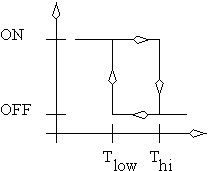
\includegraphics{HysteresisGraph}}
    \caption{A more complex furnace controller for a house.}
    \label{fig:sequentialCirHysteresisGraph}
\end{figure}

The y-axis of this graph describes the state of the furnace; either it is
on or it is off.  The x-axis describes the temperature of the house.  If the
house temperature is less than $T_{low}$, then the furnace is on.  If the
house temperature is greater than $T_{hi}$, then the furnace is off.  However,
when the house temperature is between $T_{hi}$ and $T_{low}$, then the
behavior of the furnace depends on what it was doing before the
temperature reached this value.  If the furnace was on, then it continues
to be on while it passes through the region $T_{low}$ to $T_{hi}$. This behavior
is the upper horizontal line with the right-facing arrow in
Figure~\ref{fig:sequentialCirHysteresisGraph}.  If the furnace was off, then it continues
to be off while in the region $T_{low}$ to $T_{hi}$.  This behavior is the
horizontal line with the left-facing arrow in Figure~\ref{fig:sequentialCirHysteresisGraph}.

The graph in Figure~\ref{fig:sequentialCirHysteresisGraph} describes a relation because
for a given $x$ value there can be more than one $y=f(x)$ value.  In order to
describe the relationship between the input and output, a variable
storing the \textit{ state} of the furnace is needed.  The output of the controller
is then a function of the input and the state.  Instead of using the graph
shown in Figure~\ref{fig:sequentialCirHysteresisGraph} to describe the behavior of the
furnace controller, digital designers utilize \textit{ state diagrams}.
\index{state diagram}

A state diagram is a diagram which describes the behavior of a sequential
circuit (a digital system with states).  In a state diagram, each of the
states is given a name and placed inside a circuit.  States are then
connected together with arcs. States \textbf{ A} and \textbf{ B} are connected together
with an arc pointing from \textbf{ A} to \textbf{ B} if there is an input which causes
the system to transition from state \textbf{ A} to state \textbf{ B}.

The furnace controller has two states, ``on" and ``off" as shown in
Figure~\ref{fig:sequentialCirHysteresisSD}.  The arc from ``on" to ``off" is labeled
$T_{hi}$ because when $T_{hi}$ is true the furnace is turned off.
The ``*" in the off state indicates that it is the reset state; the
state the system starts in when first turned on.

\begin{figure}[ht]
    \center{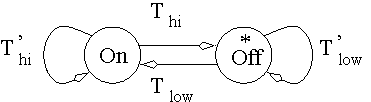
\includegraphics{HysteresisSD}}
    \caption{A state diagram describing the furnace controller of
    Figure~\ref{fig:sequentialCirHysteresisGraph}.}
    \label{fig:sequentialCirHysteresisSD}
\end{figure}

In general, when building a state diagram, visit each state
and identify the transition the system makes for every possible
input combination.  For example, ``What state should the controller go into
when it is currently in the on state and $T_{hi}$ is false and $T_{low}$ is
false?" Since this case means that the temperature is below $T_{low}$,
the furnace should stay in the on state.  Notice that this
transition is not shown in Figure~\ref{fig:sequentialCirHysteresisSD}.  This is an
instance of the general principle used in the construction of all state
diagrams; any input combination not explicitly shown on the state diagram
is assumed to not cause a change of state. This principle helps reduce the
clutter on state diagrams by removing a multitude of arcs beginning and ending
in the same state.  The state diagram in Figure~\ref{fig:sequentialCirHysteresisSD} also
exhibits two other properties, completeness and consistency, necessary
for its correctness.

\begin{description}
        \label{page:completeness}
    \item[Completeness] - The logical OR of the conditions on all the outgoing
        arcs must equal 1.  This implies that every possible combination of the
        variables used on the outgoing arcs has been described.  In other words,
        the transitions out of a state have been completely specified.  For
        example, state \textbf{ A} in Figure~\ref{fig:sequentialCirSDproperties}
        is complete because $x + x'y + x'y' = x + x'(y+y') = x + x' = 1$.  State
        \textbf{ B} in Figure~\ref{fig:sequentialCirSDproperties} is not complete because
        $x + xy + x'y' = x(1+y) + x'y' = x + x'y' \ne 1$.

    \item[Unequivocal] - The logic AND of the conditions on any pair of arcs
        must equal 0.  This implies that no pair of arcs include the same input
        condition.  If two arcs included the same input condition, then
        this would make the decision of which state to go to next ambiguous or
        equivocal.  For example, state \textbf{ A} in Figure~\ref{fig:sequentialCirSDproperties}
        is unequivocal because $(x)(x'y) = 0$, and $(x)(x'y')=0$, and
        $(x'y)(x'y') = 0$.  State \textbf{ B} in Figure~\ref{fig:sequentialCirSDproperties} is not
        unequivocal because $(x)(xy) = xy$.  If the circuit was in state \textbf{ B} and
        the input $(x,y)=(1,1)$ arrived, then the arc labeled $x$ and the arc
        labeled $xy$ are both true and would both be taken.  However, the
        circuit may only be in one state at a time, leaving it to decide which
        true condition to accept.
\end{description}

\begin{figure}[ht]
    \center{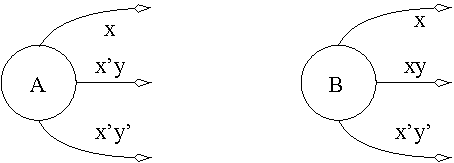
\includegraphics{SDproperties}}
    \caption{A portion of a state diagram showing two states.
        State \textbf{ A} is complete and unequivocal, while state \textbf{ B} is
    neither complete nor unequivocal.}
    \label{fig:sequentialCirSDproperties}
\end{figure}

A state diagram in which every state is complete and unequivocal
is completely unambiguous.  In every state, for any combination of
inputs, there is exactly one next state.  In order to
build machines whose behavior can be described by state diagrams,
a circuit element is needed which can store information.  These
circuit elements, called the basic memory elements, are the
sequential circuit analogy of the AND, OR, and NOT gates to
combinational logic.

\section{Basic Memory Elements}
The fundamental building blocks of sequential circuits are basic memory
elements.  A basic memory element has the ability to store one bit of
information.  This stored bit is the state of the basic memory element.
The state is always available on an output signal called $Q$.
There are a variety of basic memory elements; they are
differentiated by two fundamental characteristics:

\begin{enumerate}
    \item \textbf{ Clock} - Basic memory elements are characterized by
        when they sample their inputs.  Having tight restrictions on the
        times when a memory element can sample its inputs greatly
        simplifies the design of sequential circuits.  A \textit{ clock}
        input is used to tell the basic memory element when it should sample
        its data input(s).  A digital clock is a signal which
        changes its logic level between 0 and 1 with a fixed frequency.
        A basic memory element can be either a latch, clocked latch, or
        a flip flop.

        \begin{enumerate}

                \index{latch}
            \item Latches: A latch continuously samples its inputs.
                Latches do not have a clock input.

                \index{clocked latch}
            \item Clocked latches: A clocked latch samples its inputs when
                the clock input equals 1.  When the clock input equals 0, the
                clocked latch does not change the currently stored bit.

                \index{flip flop}
            \item Flip flops: A flip flop samples its input when the its
                clock input rises.  The clock is said to rise when it goes
                from a logic 0 to a logic 1.  When the clock input is not rising,
                the flip flop does not change the currently stored bit.
        \end{enumerate}

    \item \textbf{ Data} - Basic memory elements are characterized by
        their data inputs and how the inputs are transformed into the
        stored bit value; the clock is not considered a data input.
        A basic memory element can be either a D, T, SR, or JK device.

        \begin{enumerate}

            \item
                \marginpar{\tiny
                    \begin{tabular}{c||c}
                        D & Q+   \\ \hline
                        0 & 0 \\ \hline
                        1 & 1 \\
                    \end{tabular}
                }
                A D memory element has a single data input called $D$;
                the D stands for \textit{ data}.  When the
                D memory device samples its input, it stores this value.

            \item
                \marginpar{\tiny
                    \begin{tabular}{c||c}
                        T & Q+   \\ \hline
                        0 & Q \\ \hline
                        1 & Q' \\
                    \end{tabular}
                }
                A T memory element has a single data input called T;
                the T stands for \textit{ toggle}.  If $T=1$ when the input
                is sampled, then the T device toggles (flips) its stored bit.
                If $T=0$ when the input is sampled, then the T device holds its
                current stored bit.

            \item
                \marginpar{\tiny
                    \begin{tabular}{c|c||c}
                        S & R & Q+   \\ \hline
                        0 & 0 & Q \\ \hline
                        0 & 1 & 0 \\ \hline
                        1 & 0 & 1 \\ \hline
                        1 & 1 & x \\
                    \end{tabular}
                }
                A SR memory element has two data inputs called SR;
                the S stands for \textit{ set} and the R for \textit{ reset}.
                If $SR=00$ when the input is sampled, then the SR device retains
                its stored bit; the device \textit{ holds} its stored bit.
                If $SR=01$ when the input is sampled, then the SR device stores a 0;
                the device \textit{ resets} its stored bit.
                If $SR=10$ when the input is sampled, then the SR device stores a 1;
                the device \textit{ sets} its stored bit.
                The input of a SR device should never be set to 11.

            \item
                \marginpar{\tiny
                    \begin{tabular}{c|c||c}
                        J & K & Q+   \\ \hline
                        0 & 0 & Q \\ \hline
                        0 & 1 & 0 \\ \hline
                        1 & 0 & 1 \\ \hline
                        1 & 1 & Q' \\
                    \end{tabular}
                }
                A JK memory element has two data inputs called $J$ and $K$. They have
                no good acronym, but act very much like $S$ and $R$, respectively.
                If $JK=00$ when the input is sampled, then the JK device retains
                its stored bit; \textit{ holds}.
                If $JK=01$ when the input is sampled, then the JK device stores a 0; \textit{ resets}.
                If $JK=10$ when the input is sampled, then the JK device stores a 1; \textit{ sets}.
                If $JK=11$ when the input is sampled, then the JK device toggles its
                stored bit value; \textit{ toggles}.
        \end{enumerate}
\end{enumerate}

The information on how a basic memory element processes the input into
the stored bit is summarized in the state tables shown in the margins.
A state table is a truth table describing the changes in state
of a sequential  circuit.  Remember that the state of a basic memory
element is the value of its stored bit.  Notice the state column
is headed by $Q^+$. The ``$+$" indicates the state to be assumed
in the (very) near future.

The type of basic memory element being used in a
circuit diagram is indicated by the labels present on the data inputs and the
notation present on the clock input.  A latch does not have a clock
input, a clocked latch has the label ``clk" on its clock input,
while a flip flop's clock input has a triangular notch accompanying
the label ``clk".  Figure~\ref{fig:sequentialCirdevices} shows a D latch,
D clocked latch, and a D flip flop.  Whenever an input is accompanied
by a triangular notch it means that the input is \textit{ edge sensitive}
\index{edge sensitive}.

\begin{figure}[ht]
    \center{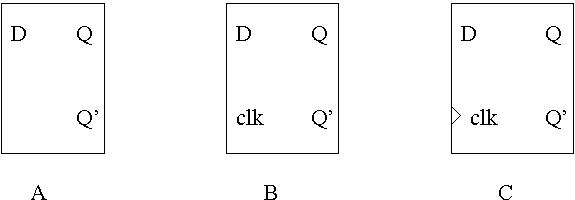
\includegraphics{devices}}
    \caption{Different symbols are used to describe \textit{ when} a basic
memory element samples its input.  A) D latch. B) D clocked latch.
C) D flip flop.}
\label{fig:sequentialCirdevices}
\end{figure}

Edge sensitive means that the input responds (or is sensitive)
to changes in the logic level of the input, not the level of the
of input.  There are two types of edge sensitive inputs, positive
and negative.  An input sensitive to positive edges responds to an
input  transition from logic 0 to 1, a positive change in the logic
level.  An input sensitive to a negative edge responds to an input
transition from logic 1 to logic 0, a negative change in the logic
level.  Input which are sensitive to negative edges have a inversion
``bubble" placed to the left of the triangular notch, like that shown
in Figure~\ref{fig:sequentialCirDFF}.

Forming every combination of the two characteristics of basic
memory elements yields 12 variations.  These variations are
organized by listing the data characteristics as column
headers and listing the clock characteristics as rows headers.
The resulting table is shown below.
\\ \\
\begin{tabular}{|c|c|c|c|}\hline
&  Latch & Clocked Latch  & Flip Flop   \\ \hline
D  &        &      &    \\ \hline
T  &        &     &    \\ \hline
SR &        &      &    \\ \hline
JK &        &     &    \\ \hline
\end{tabular}
\\ \\
While this table encompasses every possible basic memory
element, several of them are not built either because they
exhibit non-deterministic behavior or because their implementation
is trivial.  Before delving into these issues, a well-behaved basic memory
element, the D clocked latch, is examined.

\section{The D Clocked Latch}
Understanding the behavior of the D clocked latch requires
an understanding of its two characteristics, its clock
input and its data input.  Being a latch, it samples its
data inputs when the clock is 1 and holds its stored bit
when the clock is 0.  Being a D device, its sampled value
becomes the stored bit. Putting these two characteristics
together, a D clocked latch is defined as a memory
element that samples its D input continuously while the clock
equals 1, stores this value as the state, and outputs it on
the $Q$ output.  In other words, when the clock equals 1, the
$Q$ output follows the $D$ inputs. When the clock input is 0,
the D clocked latch ignores the D input and holds the value
of its stored bit.  Hence, when the clock is 0, the
$Q$ output does not change.

To better understand the behavior of the D clocked latch,
examine how the device responds to inputs through
the timing diagram in Figure~\ref{fig:sequentialCirDCL}.

\begin{figure}[ht]
\center{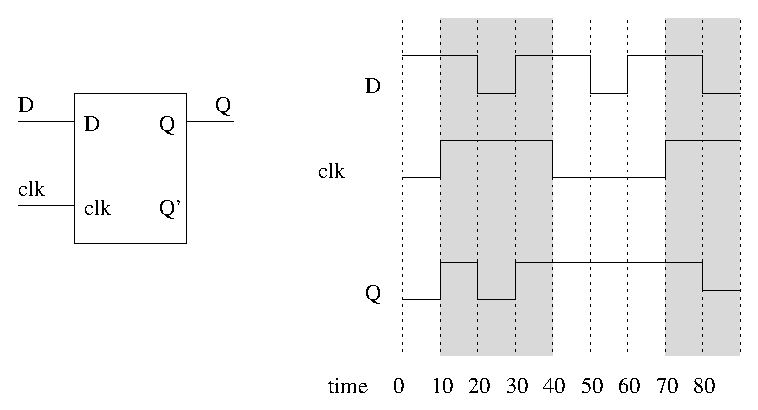
\includegraphics{DCL}}
\caption{A timing diagram showing the behavior of a D clocked latch.
The shaded regions describe when the latch samples its data inputs.}
\label{fig:sequentialCirDCL}
\end{figure}

Initially, the value of $Q$ is given as 0.  The initial value
of any basic memory element on power-up is an important issue
to be addressed later. For now, assume the
D clock latch starts off in the 0 state.  From time=0 to time=10, the
clock input is 0. Hence, $Q$ holds its value of 0.  When the
clock input goes to logic 1 at time=10, the device immediately
starts sampling the D input, storing this value as the state,
and then making the state available as the $Q$ output.  From
time=10 to time=40, the clock equals 1 and the $Q$ output follows
the D input.  From time=40 to time=70, the clock input is 0, and
the device holds its stored state, so $Q$ does not change
regardless of what D is doing.

\section{The JK Flip Flop}
The JK flip flop has two data inputs, an edge sensitive clock
input and an output $Q$, representing the stored bit.  The
JK flip flop samples its two data inputs on the rising edge
of the clock and transforms the stored bit according to the
JK's state table.  At all other times, the stored bit remains
unchanged, hence $Q$ remains unchanged.

The behavior of the JK flip flop can be better understood
by examining how it responds to inputs through time in the
timing diagram of Figure~\ref{fig:sequentialCirJKFF}.
The timing diagram of Figure~\ref{fig:sequentialCirJKFF}
is used to explain its behavior.
\begin{figure}[ht]
\center{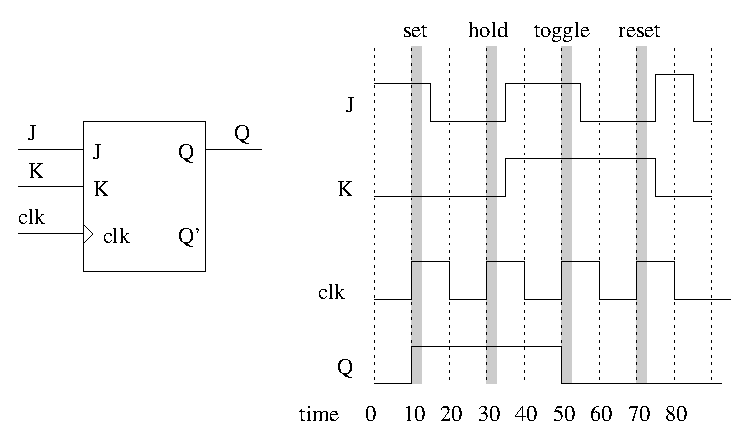
\includegraphics{JKFF}}
\caption{A timing diagram showing the behavior of a JK flip flop.}
\label{fig:sequentialCirJKFF}
\end{figure}

Since a flip flop only samples its inputs during the rising edge
of the clock input, its $J$ and $K$ values are examined
at times 10, 30, 50, 70. At all other times the stored bit, and
hence $Q$, does not change. The initial value of $Q$ is 0.  At
time=10, the clock rises, and so the inputs are sampled, $J=1$ and
$K=0$.  According to the state table, this input combination causes
the JK flip flop to sets its stored bit to 1, causing $Q$ to go
to 1 at time=10.  At the next rising edge of the clock at time=30,
$J=1$ and $K=1$, and so the JK flip flop toggles its stored bit value.
Since the stored bit was 1 before the clock edge, the stored bit
becomes 0 and $Q$ goes to 0.  The reader is invited to verify the
remainder of the timing diagram.

\section{The Negative Edge Triggered D Flip Flop}
Often, the polarity of the clock input to a
basic memory element is reversed.  For a clocked latch, this
means the data input is sampled while the clock equals 0.
For a flip flop, this means the data input is sampled on
the negative edge of the clock, when the clock transitions
from a 1 to a 0. The term ``negative edge" is used because when
drawn on a timing diagram, the slope of the clock signal is
negative.  The transition from logic 1 to logic 0 is also referred
to as a falling edge for similar reasons.
One indicates the polarity
of the clock is inverted by placing a ``bubble" in front of
the clock input on the schematic representation as shown
in Figure~\ref{fig:sequentialCirDFF}.  The bubble is reminiscent
of the bubble on the output side of an inverter and
represents inversion of the clock input. Beside the fact
that a negative edge-triggered D flip flop samples its
data input on the falling edge of the clock, it acts like
a D flip flop in all other respects.

To better understand the behavior of the negative edge-triggered
D flip flop its behavior is observed when subjected to the inputs
shown in Figure~\ref{fig:sequentialCirDFF}.

\begin{figure}[ht]
\center{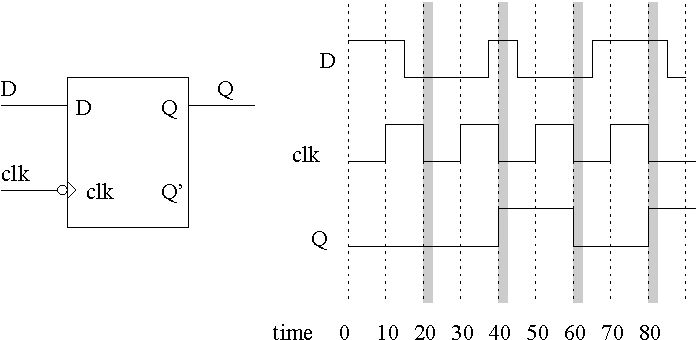
\includegraphics{DFF}}
\caption{A timing diagram showing the behavior of a
negative edge triggered D flip flop.}
\label{fig:sequentialCirDFF}
\end{figure}

The negative edge-triggered D flip flop samples its inputs on the
falling edges of the clock, at times 20, 40, 60, and 80.  Only
at these times does the stored bit take on the value of the
D input.  In other words, when the clock transitions from logic 1 to
logic 0, the D input is sampled, and then asserted on the $Q$ output.
At all other times, the $Q$ output remains unchanged.

\section{The SR Latch}
\index{latch!SR|(}
The SR latch has two data inputs, no clock input and an output $Q$,
representing the stored bit. The SR latch continuously samples
its $S$ and $R$ inputs and sets the stored bit when $S=1$, resets the
stored bit when $R=1$, and holds its stored bit when $S=0$ and $R=0$.
Since simultaneously setting and resetting the
stored bit makes no sense, the input $S=1$ and $R=1$ should never be applied to
the device.  Thus, the stored bit is a ``don't care" for this input
combination.

The behavior of the SR latch can be better understood
by examining how it responds to inputs through time in the
timing diagram in Figure~\ref{fig:sequentialCirSRLtime}.

\begin{figure}[ht]
\center{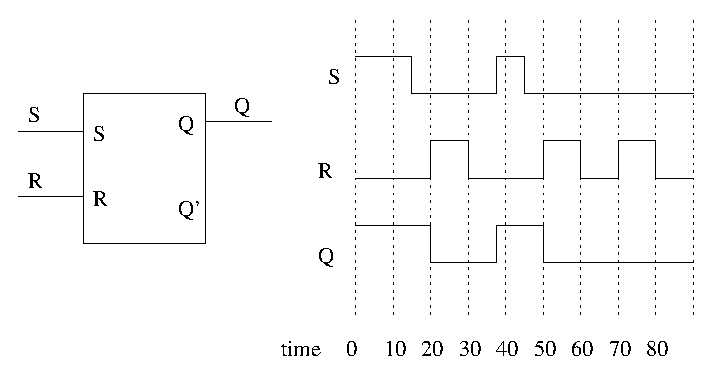
\includegraphics{SRLtime}}
\caption{A timing diagram showing the behavior of a
SR latch.}
\label{fig:sequentialCirSRLtime}
\end{figure}

Initially, at time=0, the SR latch is in a set condition, so its
stored bit and consequently its output $Q$ equals 1.  At around
time=15, both S and R go to 0, so the stored bit holds a 1.  From
time=20 to time=30, the device is being reset, so $Q$ goes to 0.  Between
time=30 and time=38, both S and R are 0, so the stored bit holds at 0.
The reader can verify the remainder of the timing diagram.
Note that at time=18 and time=32, the SR latch has the same input, both
S and R are 0.  However, the output of the device is different because
of the past history of the inputs.  In other words, the SR latch
remembers what its inputs were in the past.

The SR latch is the only basic memory element whose internal
organization will be analyzed.  The goal is to understand how
the circuit for a SR latch realizes the state table for a SR
device.

Consider the circuit realization of an SR latch
given in Figure~\ref{fig:sequentialCirSRL}.  Three important
observations can be made about this figure. First, the SR
latch is a simple circuit, sometimes referred to as cross-coupled
NORs for obvious reasons.  Second, the circuit contains feedback;
outputs are routed back to the inputs.  Feedback is an essential
feature of any system which has memory.  Third, the outputs are
labeled $Q$ and $Q'$ even though there is no inverter between the
$Q$ and $Q'$ outputs.  In most, but not all cases, these
outputs will have opposing values.

\begin{figure}[ht]
\center{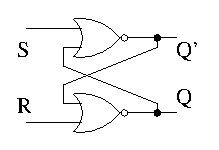
\includegraphics{SRL}}
\caption{The circuit inside a SR latch.}
\label{fig:sequentialCirSRL}
\end{figure}

The behavior of the circuit in Figure~\ref{fig:sequentialCirSRL} is governed
by the behavior of a NOR gate.  Thus, it makes sense to start with
the truth table for a NOR gate.

$$
\begin{array}{c|c||c}
A  & B  & (A+B)'  \\ \hline
0  & 0  & 1  \\ \hline
0  & 1  & 0  \\ \hline
1  & 0  & 0  \\ \hline
1  & 1  & 0  \\
\end{array}$$

From this truth table, a simple observation should be made:
Whenever the input to a NOR gate equals 1, the output equals 0.
This will be referred to as the \textit{ NOR gate heuristic}.

To understand the behavior of the circuit shown in
Figure~\ref{fig:sequentialCirSRL}, start by examining what happens when
$S=1$ and $R=0$.  According to the NOR gate heuristic, the output
associated with the top NOR gate will output 0, hence $Q'=0$.
The $Q'$ output is an input to the bottom NOR gate.  Since both
of the bottom NOR gates' inputs are 0, it outputs 1.  Hence,
$Q=1$.  Thus, when $S=1$ and $R=0$, the $Q$ output is set to 1 and
its negation, $Q'$ is 0.

The analysis of the circuits behavior when $S=0$ and $R=1$ is
identical except the roles of the top and bottom NOR gates
are interchanged.  Consequently, the device is reset causing
$Q$ to output 0 and its negation, $Q'$ to output 1.

The behavior of the circuit shown in Figure~\ref{fig:sequentialCirSRL},
is more complicated when $S=0$ and $R=0$ because the output
depends on what has happened in the past. (See time=18 and time=32
in Figure~\ref{fig:sequentialCirSRLtime}.)  Furthermore, the NOR gate
heuristic does not help, at least initially, because neither
input is 1.

In order to make some headway into the analysis, start
by assuming the SR latch is being reset ($S=0$ and $R=1$),
causing $Q=0$ and $Q'=1$.  Figure~\ref{fig:sequentialCirSRL1}A shows what
happens in the instant after the R input is changed to 0.
The inputs to the upper NOR gate, labeled TOP, are both 0.
Hence, the output of the upper NOR gate is 1, consistent with
the existing value of $Q'$.  This result causes one of the inputs to
the lower NOR gate, labeled BOT, to equal 1.  By the NOR
gate heuristic, the output of the lower NOR gate goes to 0,
consistent with the existing value of $Q$.  Thus, when the
inputs to a SR latch which is being reset are changed to
$S=0$ and $R=0$, the output remains unchanged.  Now, change this
assumption and start by setting the SR latch and see what happens
when the inputs are changed to $S=0$ and $R=0$.

If $S=1$ and $R=0$, then $Q=1$ and $Q'=0$.  Figure~\ref{fig:sequentialCirSRL1}B
shows what happens in the instant after $S=0$.  The inputs to
the upper NOR gate, labeled TOP, are 1 and 0.  By the NOR
gate heuristic, $Q'=0$, consistent with its value.  The
inputs to the lower NOR gate, labeled BOT, are both 0. Hence,
$Q=0$, consistent with its existing value of $Q$.

\begin{figure}[ht]
\center{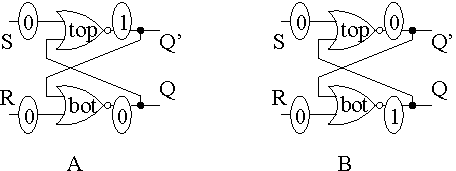
\includegraphics{SR1}}
\caption{The analysis of the SR latch when the S and R
inputs are both 0.}
\label{fig:sequentialCirSRL1}
\end{figure}

In either case when $S=0$ and $R=0$, the outputs $Q$ and $Q'$ retain
their values.  In other words, the SR latch holds its value when
both inputs are 0.
\index{latch!SR|)}

\section{Unimplemented Basic Memory Elements}
As mentioned earlier, there are some basic memory elements
which are not realized because they exhibit non-deterministic
behavior or their implementation is trivial.  The sole example
of the latter is the D latch.  \index{latch!silly}
Since it is a latch, it is continuously sampling its input.  Since it is a
D device, its sampled input is stored and output to $Q$. Hence, the
D latch continuously samples its input and outputs it to $Q$.
The D latch is nothing more than a piece of wire.

A basic memory element which exhibits non-deterministic behavior
is the  T latch. \index{latch!bad}  A T latch continuously samples
its input and updates its stored bits.  As a T device, it toggles
its stored bit when it samples $T=1$.  Unfortunately, when $T=1$,
a T latch will continuously toggle its stored bit. The problem is
there is no way to know how fast the T latch is toggling its stored
bit and consequently the state of the stored bit after the T input
returns to 0 is undetermined.  Hence, a T latch exhibits
non-deterministic behavior, behavior that cannot be
determined/predicted beforehand.  The only situation when this
behavior is beneficial is for a random number generator.

Any latch or clocked latch which can be forced to continuously toggle
its stored bit exhibits non-deterministic behavior.  Consequently,
T latches, T clock latches, JK latches, and JK clocked latches are
not commonly constructed.  However, T flop flops and JK flips flops
are constructed because they do not continuously sample their inputs,
because the clock edge is a singular event.  Hence, these two devices
sample their inputs once (per clock edge) and toggle at most
one time (per clock edge).

\section{Flip Flop Details}
There are two issues that have, up till now, been ignored
that must now be addressed.  The first involves
the possibility of changing the data input of a flip flop at the
same time as the clock input.  The second involves the initial
value of a basic memory element at power-up. The first question
is now examined.

What would happen if the D input to a D flip flop were changed at
the same time the clock signal changed?  Since flip flops are
real devices, the answer is that the stored bit will be
undetermined because the sample taken could be prior to,
or after, the clock edge.  In order to avoid the problem,
manufacturers of flip flops specify a region of time, before and
after the clock edge, during which changes to the data input are
prohibited.  Changing the data input in the prohibited region
may result in the stored bit being undetermined.

Setup time, \index{setup time} \label{page:setup} denoted $T_{su}$, is the
amount of time before the rising edge of the clock when the data
inputs must be stable, graphically illustrated in
Figure~\ref{fig:sequentialCirff-time}.  Hold time, \index{hold time} denoted $T_h$,
is the amount of time after the rising edge of the clock when the data
input must be stable.  Finally, propagation delay, denoted $T_p$,
\index{propagation delay!flip flop} \index{flip flop!propagation delay}
is the amount of time after the rising edge of the clock required for the
new $Q$ value to become valid.

\begin{figure}[ht]
\center{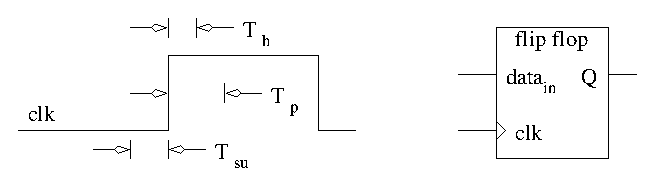
\includegraphics{ff-time}}
\caption{The significant time intervals for flip flop inputs and outputs.}
\label{fig:sequentialCirff-time}
\end{figure}

Typical values for a D flip flop are shown in the following
table.  Notice the propagation delay is longer than the hold time.
This characteristic makes it possible to cascade flip flops, that is, to
run the $Q$ output of one flip flop into the data input of a second
flip flop.  Since $T_p > T_h$, the hold time of the second flip flop
will be completed before the first flip flop changes its value.
\label{page:FFdelay}

\begin{tabular}{c|c}
Quantity & Time \\ \hline
$T_{su}$ & 20nS  \\ \hline
$T_h$    & 5nS  \\ \hline
$T_p$    & 15nS  \\
\end{tabular}

Of the three times associated with a flip flop, only the setup
time is relevant to the design of the circuits in this text.
The only situation where the setup time is needed is to determine
the maximum clocking frequency of a circuit.  When doing so,
the clocking frequency must be set slow enough to allow all the
inputs to the flip flops to stabilize prior to clocking them.  This
problem will be taken up in a latter chapter.  This section will
finish by examining the second problem mentioned at the beginning
of this section, namely, what is the value of the stored bit at power-up?

When a basic memory element is powered-up, it has no previous history
and consequently its stored bit is undefined until one is assigned to
the device.  To address this problem, manufacturers often equip
basic memory elements with \index{flip flop!asynchronous set, reset}
asynchronous active low set and
asynchronous active low reset inputs, shown at the top
and bottom on the D flip flop in Figure~\ref{fig:sequentialCirDFFSR}
as $S$ and $R$ respectively.

\begin{figure}[ht]
\center{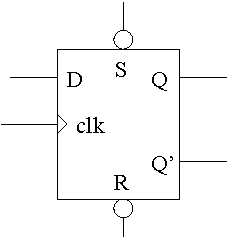
\includegraphics{DFFSR}}
\caption{A D flip flop with asynchronous active low set and asynchronous
active low reset inputs, labeled $S$ and $R$ respectively.}
\label{fig:sequentialCirDFFSR}
\end{figure}

To understand what these inputs do, examine each word in its
name in turn.  \textit{ Asynchronous} means that the $S$ and $R$ inputs
function without regard to the clock.  \textit{ Active low} means that these
inputs elicit their behavior when the signal value equals 0.  \textit{ Set
and reset} means that these inputs either set $Q=1$ or reset $Q=0$.
Thus, when $R=1$, the output is $Q=0$ -- regardless of what the clock is doing.
Consider the $S$ and $R$ inputs to have the highest priority
of all the inputs to the flip flop.  That is, when $R$ is pulled
low, the $Q$ output immediately goes to logic 0, every other input
is ignored, and stays there as long as R=0.

Normally, all the asynchronous active low reset lines in a digital
system are tied together in one massive reset net.  Pulling this
line low then resets all the memory elements in the circuit giving
them a known state.  If some of the memory elements should be
initialized to 1, then their asynchronous active low sets are tied
together to form a set net.  Often, the reset net (and the set net)
is connected to a special output from the system power supply.  This
power supply output holds the system in reset until the power
supply has reached its operating output voltage.
